\section{Results}\label{sec:results}

Risks in RQ3 and RQ4 are with respect to construction labels on development data. Coverage and risk use the 258 labelled pairs as denominator, and intervals are 95\% project-cluster bootstrap intervals. Numbers are for cross-validation seed~0 on the Linux-branch code unless stated otherwise. None of the analyses below was re-run for this revision; every value is read from existing machine-readable outputs (Section~\ref{sec:repro}).

\subsection{RQ1: Integrity-Checked Evidence and Reproducible Analysis}\label{sec:res-rq1}
\paragraph*{Reproducible analysis} The development records file is byte-identical on the Linux and macOS branches (same MD5). The Linux statistical evaluation reproduces the macOS pre-fix evaluation: point estimates agree to $10^{-9}$ for seeds 0--2 under both blocker policies, and intervals differ only through the number of bootstrap resamples (2{,}000 vs.\ 10{,}000). The post-hoc \ers{} matrices produced on the two platforms are identical cell for cell. The \sbg{} test suite (\code{tests/v8}) passed with 247 tests, 8 skipped and 2 expected failures on macOS at the final commit; the two expected failures are the profile-defect tests that the fix resolves.

\paragraph*{Original attack suite} The original suite contains 15 attacks against a pair whose honest verdict is \DIV{}. Before hardening, on macOS, 3 were blocked, 9 detected, 1 had no effect and 2 succeeded. The two successes were hiding a standard-output divergence by patching the harness's capture object (A08), and editing an unverified evidence field and re-binding the sidecar after recomputing the hash chain (P04). The independent capture and the anchor were introduced in response, and both attacks are now detected and force \INS{}. Four attacks were added; one of them, re-anchoring with the key (P08), succeeds by design because it is outside the threat model.

\paragraph*{Re-run at the final commit} The suite and six evaluation-awareness probes were re-executed at the final commit on macOS. Of 25 attacks and probes, 3 were blocked, 15 detected, 5 had no effect and 2 succeeded (Table~\ref{tab:security}).
\begin{itemize}
\item Of the 15 detections, 10 force \INS{} through the trust gate.
\item Five are detection only: A01, A02, A07, P06 and SENSE04c are caught only by the optional shadow or source-binding checks, and the effective verdict remains a false \NDO{}.
\item The two successes are the out-of-scope key-holder forgery (P08) and SENSE04b, which reads the variant's real path from compiled code objects and produces a false \NDO{} with no check firing. The SENSE04 fix, which sanitises \code{\_\_file\_\_} and \code{sys.argv}, is therefore partial.
\item A17 (a tee record forged with a guessed nonce) turns a true \DIV{} into \INS{}: a denial of a true divergence, not a false assurance.
\end{itemize}

\paragraph*{Linux probes} A Linux suite, run before the SENSE04 fix, contains 51 tamper probes and 74 isolation probes (named ``container'' in the result file, although no container runtime is invoked). All 51 tamper probes were detected. They comprise 24 distinct operations, and the five substitution probes were detected only through source binding. Of the 74 isolation probes:
\begin{itemize}
\item 8 left the true verdict intact;
\item 1 (SENSE04) produced a false \NDO{};
\item 65 ended in \INS{} with no recorded cause, after about 0.2\,s each instead of the 0.7--3.1\,s of runs that reached a decision. They include probes that should have produced \DIV{}.
\end{itemize}
The 65 undecided runs are fail-safe but are not evidence of isolation. The Linux results file records no host, sandbox configuration or timestamp.

\paragraph*{Answer to RQ1} Within threat model A1--A3, the verified position is:
\begin{itemize}
\item fail-safe integrity against keyless post-hoc writers;
\item prevention of result-channel attacks and of the tested standard-output tampering;
\item detection, but not prevention, of in-process harness forgery and evidence substitution;
\item at least one open evaluation-awareness channel.
\end{itemize}
The statistical analysis reproduces across platforms because it is a deterministic function of identical records. This establishes reproducibility of the \emph{analysis}, not of evidence \emph{collection} on two platforms.

% Sources: research/v8-mac-hardening results/v8_mac_security/attack_suite_{before,after}.json; audit/security_rerun_darwin.json;
% results/v8/linux/expanded_security_suite_results.json; classification in audit/security_outcomes.json (scripts/build_security_outcomes.py).
\begin{table}[!t]
\caption{Adversarial evaluation outcomes. Controls excluded. ``Det.\ only'' counts detections by optional reviewer checks that leave a false \NDO{} as the effective verdict.}
\label{tab:security}
\centering
\scriptsize
\setlength{\tabcolsep}{2.2pt}
\begin{tabular}{|L{2.15cm}|c|c|c|c|c|c|}
\hline
Suite (platform) & $n$ & Blocked & \makecell{Detected\\(det.\ only)} & \makecell{No\\effect} & Succ. & \makecell{\INS{},\\cause\\unrec.} \\
\hline
Original, before hardening (macOS) & 15 & 3 & 9 (4) & 1 & 2 & -- \\
Original + hardening attacks, after (macOS) & 19 & 3 & 14 (4) & 1 & 1 & -- \\
Re-run at final commit incl.\ sensing probes (macOS) & 25 & 3 & 15 (5) & 5 & 2 & -- \\
Tamper probes (Linux) & 51 & 0 & 51 (5) & 0 & 0 & -- \\
Isolation probes (Linux, pre-fix) & 74 & 0 & 0 & 8 & 1 & 65 \\
\hline
\end{tabular}
\\[2pt]
\parbox{\columnwidth}{\scriptsize The 51 Linux tamper probes comprise 24 distinct operations. The 65 Linux isolation probes recorded as \INS{} carry no cause, completed in about 0.2\,s, and include probes that should have produced \DIV{}; they are fail-safe but are not evidence of isolation. No post-remediation Linux re-run artifact exists.}
\end{table}



\subsection{RQ2: Conformance to the Evidence Response Signature}\label{sec:res-rq2}
Table~\ref{tab:ers} reports the property matrix on all 312 development records for six predictors.

\paragraph*{The matrix detected a profile defect} The all-feature probe is an unfitted model that reads every profile feature with its declared sign. It failed irrelevant-evidence invariance (P2) on 109 of 227 applicable records: appending two inputs that reach only unchanged lines \emph{lowered} its risk by up to 0.32. The cause was the profile, whose quantity and diversity features counted inputs that reach no changed unit. After the fix (Section~\ref{sec:approach}), the probe passed P2 on all 227 records with $\Delta$ exactly zero, and no other cell changed. The fitted model passed P2 throughout, but only because it retains essentially one feature (\code{mu\_min}) that irrelevant inputs cannot move. The defect would have surfaced in any model using the quantity features, and no aggregate metric revealed it, because it changes no prediction of the fitted model on unperturbed data.

\paragraph*{The execution-level analogue corroborates the defect} In the exploratory real-execution run (Section~\ref{sec:ers}), real irrelevant inputs could be found for 7 of 30 pairs; for the rest, no seeded candidate exercised only unchanged code. On those 7, the probe failed P2 five times, with risk reductions of 0.087--0.095, and every other predictor passed. All six predictors passed the real P5 analogue on all 30 pairs. A label-blind generator found a discriminating input (real P6) for none of the 20 primary pairs and for 1 of the 10 supplementary pairs, which passed. The analogue therefore reproduces the post-hoc defect under real execution, but it is too small to test P6.

\paragraph*{The matrix separates decision procedures} Replaying the recorded V7-B verdict fails divergence responsiveness (P6) on 71 records; its 157 passes rest entirely on stored \INS{} verdicts, that is, on abstention credit. It also fails integrity rejection (P8) on 155 records, because a stored verdict cannot react to new evidence. Re-applying the V7-B gate to the perturbed record repairs P6 but still fails P8 on 84 records. Every one of these is a witnessed divergence that V7-B keeps as \DIV{} on evidence marked as tampered. The \sbg{} trust gate passes P8 on all 312 records by construction; it was added after a first run of the matrix showed the same 84 failures for an earlier \sbg{} procedure.

\paragraph*{Responses are real but concentrated} No monotone pass of the fitted model rests on abstention credit. Its risk rose beyond tolerance in 9 of 16 P1 trials, 68 of 93 P1b trials and 100 of 176 P5 trials, and was unchanged for P4, P7 and P9. The model therefore responds to the loss of relevant evidence and to reduced reproducibility. It is indifferent to channel loss, provenance and environment, because those features were constant in training.

\paragraph*{Answer to RQ2} The matrix found one real estimator defect, corroborated under real execution, and exposed the predecessor's integrity blindness. For the fitted model, the passes on P4, P7 and P9 are vacuous.

% Source: results/v8/linux/perturb/posthoc_matrix.{json,md} (Linux branch, pre-fix profile) and, for the probe after the profile fix,
% research/v8-mac-hardening@b9b8a86c:results/v8_mac_perturb_profilefix2/posthoc_matrix.md. Driver: experiments/v8/run_perturbation_validation.py.
\begin{table*}[!t]
\caption{\ers{} property matrix on the 312 development records (post-hoc perturbations of recorded evidence). Each cell gives the number of passes among the applicable trials; N/A trials are excluded. ``Resp.'' is the number of applicable trials in which the fitted model's risk moved by more than the tolerance. Failures are in bold.}
\label{tab:ers}
\centering
\footnotesize
\setlength{\tabcolsep}{4pt}
\begin{tabular}{|l|l|c|c|c|c|c|c|c|c|}
\hline
 & & & \multicolumn{2}{c|}{Fitted profile model} & \multicolumn{2}{c|}{All-feature probe} & & \multicolumn{2}{c|}{V7-B gate} \\
Id & Property & Applicable & Pass & Resp. & Pre-fix & Post-fix & Activation stub & Recorded & Recomputed \\
\hline
P1 & Relevant-evidence sensitivity & 16 & 16 & 9 & 16 & 16 & 16 & 16 & 16 \\
P1b & Relevant-evidence sensitivity & 93 & 93 & 68 & 93 & 93 & 93 & 93 & 93 \\
P2 & Irrelevant-evidence invariance & 227 & 227 & 0 & \textbf{118} & 227 & 227 & 227 & 227 \\
P3 & Duplicate-evidence invariance & 262 & 262 & 0 & 262 & 262 & 262 & 262 & 262 \\
P4 & Observation-loss sensitivity & 178 & 178 & 0 & 178 & 178 & 178 & 178 & 178 \\
P5 & Reproducibility sensitivity & 176 & 176 & 100 & 176 & 176 & 176 & 176 & 176 \\
P6 & Divergence responsiveness & 228 & 228 & 0 & 228 & 228 & 228 & \textbf{157} & 228 \\
P7 & Provenance sensitivity & 178 & 178 & 0 & 178 & 178 & 178 & 178 & 178 \\
P8 & Integrity sensitivity & 312 & 312 & 0 & 312 & 312 & 312 & \textbf{157} & \textbf{228} \\
P9 & Environment sensitivity & 228 & 228 & 0 & 228 & 228 & 228 & 228 & 228 \\
\hline
\end{tabular}
\\[3pt]
\parbox{\textwidth}{\scriptsize Fitted model: $L_2$ logistic regression on the full profile, with a diagnostic threshold at the 30th percentile of in-sample eligible risk so that \NDO{} verdicts exist to be withdrawn; it is not a deployment threshold, and no pass in this column rests on abstention credit. All-feature probe: an \emph{unfitted} model that reads every profile feature with its pre-declared sign; it exists because the fitted model retains essentially one feature (\code{mu\_min}), which makes invariance checks on the other features vacuous for it. Post-fix: after restricting features to relevant evidence and collapsing unflagged copies (mac-hardening branch, commit \code{b9b8a86c}); only the P2 row changed for any predictor. Activation stub: risk $=1-a(\Ev)$. V7-B ``recorded'' replays the stored verdict and therefore ignores the perturbed evidence by construction; ``recomputed'' re-applies the V7-B gate to the perturbed record.}
\end{table*}


\subsection{RQ3: Observed False-Assurance Risk of Decision Rules}\label{sec:res-rq3}
The upper block of Table~\ref{tab:ablation} and the point markers in Fig.~\ref{fig:riskcov} show the rule baselines.
\begin{itemize}
\item \emph{Plain differential testing (B1)} issues \NDO{} on 183 of 258 labelled pairs (coverage 0.709). Of these, 31 have $Y{=}1$: an observed risk of 0.169 [0.086, 0.354]. Roughly one in six ``no difference'' outcomes concealed a labelled behavioural change. Requiring deterministic witnesses (B2) changes nothing.
\item \emph{The V7-B gate (B3)} issues 61 verdicts (coverage 0.236), 13 of them wrong: a risk of 0.213 [0.090, 0.457]. Abstaining on two thirds of the B1 verdicts (122 of 183) did not lower the risk among those that remained.
\item \emph{Coverage gates.} B4 issues 141 verdicts at 0.121 [0.044, 0.343], and B5 issues 144 at 0.125 [0.052, 0.343].
\end{itemize}
All intervals overlap substantially. Counting unlabelled \NDO{} pairs as false assurances gives worst-case risks of 0.333 (B1), 0.324 (B3), 0.225 (B4) and 0.227 (B5).

\paragraph*{Answer to RQ3} By Proposition~\ref{prop:random}, the expected risk of random abstention equals B1's 0.169 at any coverage. The gate's extra blocking removed many verdicts without removing a disproportionate share of wrong ones: it lowered the number of false assurances from 31 to 13 but not their rate. The ordering among the coverage rules is suggestive only.

\begin{table*}[!t]
\caption{Development-set comparison of SBG V8 decision rules, calibrated models and ablations (seed 0, out-of-fold).}
\label{tab:ablation}
\centering
\footnotesize
\begin{tabular}{|l|c|c|c|c|c|c|}
\hline
Method & Coverage & \#NDO & FA risk [95\% CI] & Brier & Log loss & Cal.\ slope \\
\hline
\multicolumn{7}{l}{\emph{Rule baselines (all 258 labelled pairs; policy-independent)}} \\
Plain differential testing (B1) & 0.709 & 183 & 0.169 [0.086, 0.354] & -- & -- & -- \\
B1 + repetition (B2) & 0.709 & 183 & 0.169 [0.086, 0.354] & -- & -- & -- \\
V7-B sufficiency gate (B3) & 0.236 & 61 & 0.213 [0.090, 0.457] & -- & -- & -- \\
Coverage-only gate (B4) & 0.547 & 141 & 0.121 [0.044, 0.343] & -- & -- & -- \\
Coverage-gated B1 (B5) & 0.558 & 144 & 0.125 [0.052, 0.343] & -- & -- & -- \\
Random abstention (B6)$^\dagger$ & 0.236 & 61 & 0.169 & -- & -- & -- \\
\hline
\multicolumn{7}{l}{\emph{Soft blockers (v8.0): 85 eligible labelled pairs}} \\
Coverage-only calibration (B7) & 0.236$^\ast$ & 61 & 0.230 [0.108, 0.465] & 0.225 & 0.649 & -1.83 \\
\quad + multiplicity & 0.236$^\ast$ & 61 & 0.292 [0.151, 0.471] & 0.219 & 0.637 & -0.03 \\
Multiplicity only & 0.236$^\ast$ & 61 & 0.295 [0.151, 0.473] & 0.212 & 0.620 & 0.21 \\
CEC without ERS (B9) & 0.236$^\ast$ & 61 & 0.292 [0.151, 0.468] & 0.221 & 0.645 & -0.02 \\
CEC with ERS (B8) & 0.236$^\ast$ & 61 & 0.213 [0.124, 0.392] & 0.207 & 0.615 & 0.30 \\
\hline
\multicolumn{7}{l}{\emph{Strict blockers (v8.0s $\equiv$ v8.1): 61 eligible labelled pairs}} \\
Coverage-only calibration (B7) & 0.236$^\ast$ & 61 & 0.213 [0.129, 0.473] & 0.205 & 0.615 & -4.42 \\
\quad + multiplicity & 0.236$^\ast$ & 61 & 0.213 [0.130, 0.446] & 0.188 & 0.583 & -0.11 \\
Multiplicity only & 0.236$^\ast$ & 61 & 0.213 [0.129, 0.446] & 0.189 & 0.587 & -0.17 \\
CEC without ERS (B9) & 0.236$^\ast$ & 61 & 0.213 [0.130, 0.446] & 0.188 & 0.583 & -0.11 \\
CEC with ERS (B8) & 0.236$^\ast$ & 61 & 0.213 [0.125, 0.443] & 0.182 & 0.578 & 0.05 \\
\hline
\end{tabular}
\\[2pt]
\parbox{\textwidth}{\scriptsize DEVELOPMENT DATA, EXPLORATORY, NOT INDEPENDENT VALIDATION. Split: development only (312 pairs, 258 with construction labels, 54 unlabelled and excluded, 101 labelled projects, 114 overall; quixbugs = 43.8\% of labelled pairs). Coverage and FA risk are over the 258 labelled pairs; 95\% CIs are percentile project-cluster bootstrap intervals (10{,}000 resamples). $^\ast$Model rows are rank-matched to the V7-B gate coverage $c^*=61/258$ (transductive diagnostic, not a deployable threshold); with nested-CV thresholds at $\alpha\in\{0.10,0.15\}$ the models issue 0 NDO (multiplicity-only: 1). Under strict blockers every model issues exactly V7-B's 61 NDO pairs, so risks are identical by construction; their CIs use only the ${\approx}50\%$ of resamples in which $c^*$ is attainable and are therefore not reliable. Brier, log loss and slope are on eligible pairs only (out-of-fold base-rate Brier 0.230 soft, 0.205 strict). $^\dagger$Expected risk of random abstention among B1-issuable pairs. Per-method runtime was not recorded; the whole 13-system evaluation took 109--117\,s per seed (Linux run). Linux-branch code, before the mac-branch ERS profile fix.}
\end{table*}


\begin{figure}[!t]
\centering
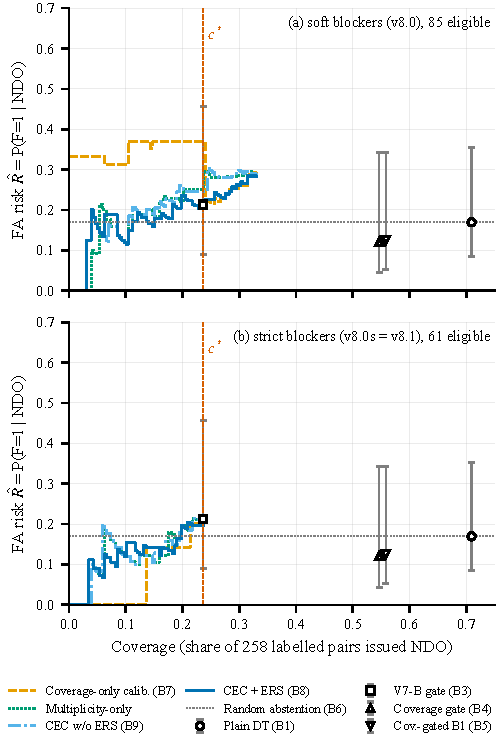
\includegraphics[width=\columnwidth]{figures/fig_risk_coverage.pdf}
\caption{Risk--coverage curves for the calibrated models (out-of-fold, seed~0) under (a) soft and (b) strict blocker policies, with rule baselines as points (95\% project-cluster bootstrap intervals). The vertical line marks $c^\ast=61/258$. Calibrated curves end at the eligible share (85 soft, 61 strict).}
\label{fig:riskcov}
\end{figure}

\subsection{RQ4: Incremental Value of \cec{} and \ers{} at Matched Coverage}\label{sec:res-rq4}
Table~\ref{tab:stats} lists every contrast with its effect, interval, one-sided $p$ and Holm-adjusted $p$. Fig.~\ref{fig:forest} plots them.

\paragraph*{Matched-coverage risk} At $c^\ast$ under the soft policy, B8 has risk 0.213 [0.124, 0.392], against 0.230 for B7, 0.292 for B9 and 0.295 for multiplicity alone. The primary contrast, B7 minus B8, is $+1.6$ points [$-6.6$, $+16.3$], so H2 is not supported. B8 ties the V7-B gate (0.0 [$-6.2$, $+16.2$]; defined in only half of the resamples) and lies 4.4 points above random abstention ($-4.4$ [$-11.5$, $+9.7$]). In the pre-registered three-test family, the Holm-adjusted $p$ is at least 0.46 in every soft-policy seed. In the eight-contrast family, the smallest Holm-adjusted $p$ is 0.68 (soft) and 1.0 (strict).

Under the strict policy every calibrated model is confined to V7-B's own 61 \NDO{} pairs. At $c^\ast$ all of them therefore issue that set, with identical risk 0.213. The strict matched contrasts are zero by construction, and their intervals (defined in about half of the resamples) are not interpreted.

\paragraph*{Probabilistic accuracy} On the 85 soft-eligible pairs, B8 has the lowest out-of-fold Brier score (0.207) and log loss (0.615) of the calibrated models, against an out-of-fold base-rate Brier score of 0.230. The profile improves log loss over coverage-only calibration by $+0.003$ [$-0.083$, $+0.058$] (H1a), and \ers{} features improve it by $+0.030$ [$-0.014$, $+0.085$] (H3). Neither interval excludes zero. On the mac-hardening branch, a placebo test that permutes the \ers{} features 100 times placed the observed gain above the 95th permutation percentile in five of six policy--seed runs ($p$ 0.01--0.03; $p=0.21$ in the sixth). We regard this as weak, unadjusted evidence that the responses carry some signal, which is insufficient to establish a predictive advantage.

\paragraph*{Calibration and deployable thresholds} Calibration slopes are unstable at this sample size (Fig.~\ref{fig:calibration}): 0.30 [$-0.46$, 1.13] for B8, and $-1.83$ for B7, whose out-of-fold ordering is inverted. When thresholds are chosen as specified (Algorithm~\ref{alg:cec}), no calibrated model issues any \NDO{} at $\alpha\in\{0.10,0.15\}$, except multiplicity-only, which issues one. A frozen-threshold study on the mac-hardening branch applied thresholds fitted on training projects to held-out projects. The conservative rule again issued nothing, and a point-estimate rule produced held-out risks of 0.24--0.50 against targets of 0.10--0.20. No calibrated model achieved risk control.

\paragraph*{Seeds, profile fix and power}\label{sec:res-robust}
\begin{itemize}
\item \emph{Seeds.} Across five seeds the primary difference is $+1.6$, $+1.6$, $+3.3$, $-4.1$ and $-4.9$ points (mean $-0.5$); its sign is unstable. The \ers{} log-loss gain ranges from 0.005 to 0.030 and includes zero in all soft-policy seeds.
\item \emph{Profile fix.} Re-running with the fixed profile (mac-hardening branch) left soft seeds 0 and 1 unchanged, moved seed~2's primary difference from $+3.3$ to $0.0$, and changed \ers{} log-loss gains by at most 0.008.
\item \emph{Power.} The 61 reference \NDO{} verdicts fall into 34 clusters, with an intra-cluster correlation of 0.61, a design effect of 1.48 and an effective sample size of about 41. The minimum detectable paired difference at 80\% power is 13.5, 16.5 and 21 points at discordant shares of 0.10, 0.15 and 0.25 (Fig.~\ref{fig:power}). Detecting 5 points would need about 460, 690 or 1{,}160 issued verdicts, 8 to 19 times the present set.
\end{itemize}

\paragraph*{Answer to RQ4} The incremental predictive value of \cec{} and \ers{} over coverage-only calibration is \emph{not demonstrated}. Because the study could detect only differences of about 16 points, this negative result is inconclusive rather than evidence of no effect.

\begin{table*}[!t]
\caption{Statistical results (soft policy, seed~0, out-of-fold). Risk effects are differences in observed false-assurance risk in percentage points; log-loss effects are differences in nats. Positive values favour B8. Intervals: 95\% paired project-cluster bootstrap (10{,}000 resamples; B6 contrast from the saved Linux run, 2{,}000 resamples). $p$: one-sided bootstrap. Holm: within the eight-contrast family; the B6 contrast belongs to the pre-registered three-test family (Holm $p=1.0$). ``Valid'': share of resamples in which the contrast is defined.}
\label{tab:stats}
\centering
\footnotesize
\setlength{\tabcolsep}{4pt}
\begin{tabular}{|l|l|c|c|c|c|c|l|}
\hline
Contrast & Hypothesis & Effect & 95\% CI & $p$ & Holm $p$ & Valid & Reading \\
\hline
\multicolumn{8}{|l|}{\emph{Matched-coverage risk at $c^\ast=0.236$ (61 verdicts)}} \\
B7 $-$ B8 & H2 (primary) & $+1.6$ & [$-6.6$, $+16.3$] & 0.42 & 1.00 & 0.999 & Not supported; below 5-pt margin \\
B3 $-$ B8 & primary family & $0.0$ & [$-6.2$, $+16.2$] & 0.33 & 1.00 & 0.502 & Tie with predecessor \\
B6 $-$ B8 & primary family & $-4.4$ & [$-11.5$, $+9.7$] & 0.76 & 1.00$^{a}$ & 1.000 & Not better than chance \\
B9 $-$ B8 & H3 (matched) & $+7.9$ & [$-2.8$, $+14.7$] & 0.09 & 0.68 & 0.999 & Inconclusive \\
Mult.\ only $-$ B8 & ablation & $+8.2$ & [$-2.5$, $+15.6$] & 0.08 & 0.68 & 0.999 & Inconclusive \\
\hline
\multicolumn{8}{|l|}{\emph{Out-of-fold log loss (85 eligible pairs)}} \\
B7 $-$ B9 & H1a & $+0.003$ & [$-0.083$, $+0.058$] & 0.45 & 1.00 & 1.000 & Not supported \\
B9 $-$ B8 & H3 & $+0.030$ & [$-0.014$, $+0.085$] & 0.08 & 0.68 & 1.000 & Not supported \\
B7 $-$ B8 & -- & $+0.033$ & [$-0.055$, $+0.104$] & 0.20 & 1.00 & 1.000 & Inconclusive \\
Mult.\ only $-$ B8 & ablation & $+0.004$ & [$-0.047$, $+0.052$] & 0.42 & 1.00 & 1.000 & Inconclusive \\
\hline
\end{tabular}
\\[3pt]
\parbox{\textwidth}{\scriptsize $^{a}$Pre-registered three-test family. Strict policy: all matched-coverage contrasts are $0$ by construction (valid share 0.502); log-loss contrasts B7$-$B9 $+0.032$ [$-0.093$, $+0.154$] and B9$-$B8 $+0.005$ [$-0.068$, $+0.090$], all Holm $p=1.0$. Worst-case and complete-case risks for the rule baselines are given in Section~\ref{sec:res-rq3}. Source: \code{audit/stats\_summary.json}.}
\end{table*}

\begin{figure}[!t]
\centering
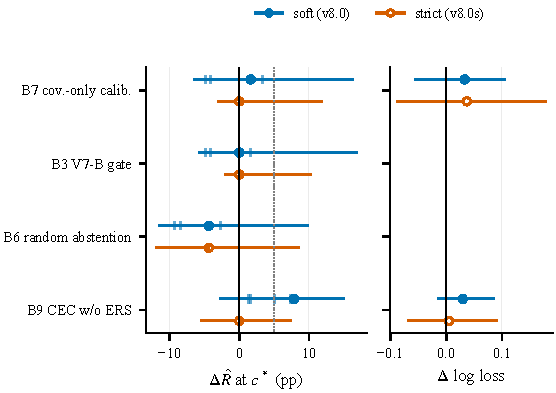
\includegraphics[width=\columnwidth]{figures/fig_ablation_forest.pdf}
\caption{Paired contrasts with full \cec{} (B8) at matched coverage $c^\ast$ (left, percentage points) and in out-of-fold log loss (right). Positive values favour B8. Dots: seed~0 with 95\% project-cluster bootstrap intervals; ticks: seeds 1--4. The dotted line marks the 5-point margin of H2. Strict-policy matched-risk intervals use only resamples in which $c^\ast$ is attainable and are shown for completeness only.}
\label{fig:forest}
\end{figure}

\begin{figure}[!t]
\centering
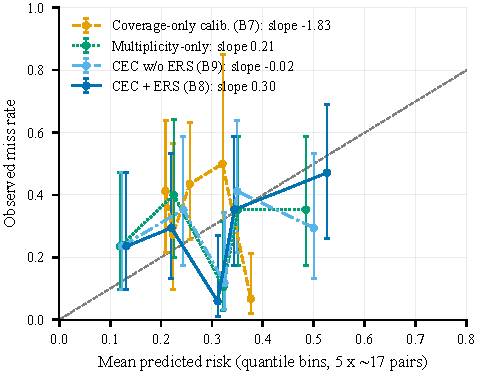
\includegraphics[width=\columnwidth]{figures/fig_calibration.pdf}
\caption{Reliability diagram for the calibrated models (soft policy, seed~0, out-of-fold, five quantile bins of about 17 eligible pairs, Wilson 95\% intervals). Legend values are logistic calibration slopes.}
\label{fig:calibration}
\end{figure}

\begin{figure}[!t]
\centering
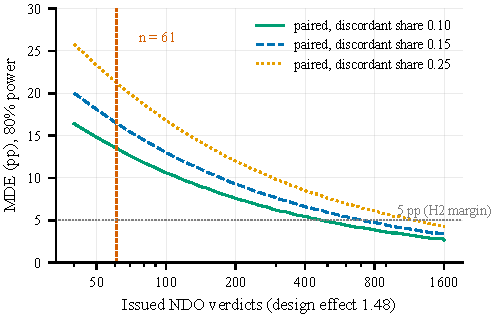
\includegraphics[width=\columnwidth]{figures/fig_power_mde.pdf}
\caption{Minimum detectable paired difference in false-assurance risk (80\% power, two-sided $\alpha=0.05$, design effect 1.48) as a function of the number of issued \NDO{} verdicts. The vertical line marks the present $n=61$; the dotted line marks the 5-point margin of H2.}
\label{fig:power}
\end{figure}

\subsection{RQ5: Scope of the Evaluation Evidence}\label{sec:res-rq5}
\paragraph*{Executed settings} Table~\ref{tab:benchmarks} lists five executed evaluation settings (A--E). Their breadth is real but narrow. The 312 program pairs come from 101 synthetic programs, 31 QuixBugs programs and 43 BugsInPy bugs in 12 projects, all executed by the collector with exit status~0. The BugsInPy units are the only real-project changes. They have no labels, so they enter RQ2 and the descriptive analyses but not the risk estimates. Under the predecessor's gate they received 6 \DIV{}, 8 \NDO{} and 32 \INS{} verdicts, an abstention rate of 70\%, against 47\% (125 of 266) in the labelled arms. Real-project changes thus pose the sufficiency problem more often, which is consistent with the motivation but is not a risk estimate. Everything is single-language, development-exposed and unadjudicated, and no benchmark was held out.
\paragraph*{The five-dataset artifact} A static audit of the artifact's generator code and manifests (\code{scripts/verify\_five\_dataset.py}) found the following:
\begin{itemize}
\item all 250 records come from 12 hand-written templates;
\item the commit identifiers are SHA-1 digests of literal strings;
\item none of the 180 Java records was compiled or run;
\item each input's outcome is set from the pair's label in \code{executor.pair\_to\_evidence\_record};
\item the integrity flag and the Linux environment identifier are hard-coded;
\item the activation-stub predictor was used;
\item six records are duplicates.
\end{itemize}
Every verdict therefore equals its label by construction, and the artifact establishes only that the record schema, profile, \ers{} harness and prediction lock process 250 records end to end. It provides no evidence about detection, false-assurance risk, cross-dataset generalisation or container isolation. Table~\ref{tab:benchmarks} (row F) and Fig.~\ref{fig:landscape}(c) present it on that basis. Under the five benchmark names the artifact holds 50, 50, 50, 50 and 50 records with 10, 10, 10, 10 and 7 project names; five of the ten BugsInPy names are not BugsInPy projects. No per-dataset metric is reported.

\paragraph*{Cross-platform evidence} Table~\ref{tab:xplat} separates what was executed on each platform from what is asserted only in report text.
\begin{itemize}
\item \emph{Both platforms:} the statistical analysis and the pre-fix \ers{} matrix, with identical results on identical records.
\item \emph{macOS only:} the profile fix, the placebo and frozen-threshold studies, the real-execution \ers{} analogue, the test suite and the security re-run at the final commit.
\item \emph{Linux, partially:} tamper and isolation probes whose result file lacks host metadata, and in which most isolation runs did not reach a decision.
\item \emph{Report text only, not used:} container-runtime isolation and a 608-test Linux regression run.
\end{itemize}
The 312 development records carry a single environment identifier and do not record the collection platform.

\paragraph*{Answer to RQ5} The evaluation spans five executed settings, including real changes from 12 BugsInPy projects, but only synthetic and QuixBugs pairs carry labels, and all data are development data in one language. There is no held-out or multi-dataset benchmark evaluation; the five-dataset artifact is template-generated and excluded. The cross-platform evidence shows that the analysis is reproducible, plus partial Linux security testing; it does not show cross-platform evidence collection.

\begin{table}[!t]
\caption{Cross-platform summary. Ex.\ = executed with raw output; Part.\ = executed but raw output incomplete; Rep.\ = report text only (not used); -- = not run.}
\label{tab:xplat}
\centering
\scriptsize
\setlength{\tabcolsep}{2.5pt}
\begin{tabular}{|L{3.4cm}|c|c|L{2.3cm}|}
\hline
Activity & macOS & Linux & Evidence \\
\hline
Evidence collection (312 pairs) & \multicolumn{2}{c|}{one env.\ id} & Platform not recorded \\
Statistics, 5 seeds $\times$ 2 policies & Ex. & Ex. & Agree to $10^{-9}$ \\
\ers{} matrix, pre-fix & Ex. & Ex. & Identical \\
Real-execution P2/P5/P6 (30 pairs) & Part. & -- & Run dirs absent \\
Profile fix; \ers{} re-run & Ex. & -- & Mac branch \\
Placebo; frozen thresholds & Ex. & -- & Mac branch \\
Test suite & Ex. & Rep. & 247 / 8 / 2 (mac) \\
Attack suite (19) & Ex. & -- & Before / after \\
Sensing probes & Ex. & Part. & Mac re-run at HEAD \\
Tamper probes (51) & -- & Part. & No host metadata \\
Isolation probes (74) & -- & Part. & 65 undecided \\
Container runtime isolation & -- & Rep. & Not invoked by code \\
\hline
\end{tabular}
\end{table}

